\chapter{Appendix A}

\section{Additional Figures}

\begin{figure}[htpb]
    \centering
    \includesvg[width=0.75\linewidth]{Figures/C_P vs. 0° Angle of Attack.svg}
    \caption[Plot of the Coefficient of pressure in relationship to the normalized x component at a Angle of attack of 0 degrees]{Plot of the \gls{C_P} in relationship to the normalized $x$ component at a \acrshort{aoa} of \qty{0} {\degree}.}
    \label{fig:C_P vs. 0° Angle of Attack.svg}
\end{figure}

\begin{figure}[htpb]
    \centering
    \includesvg[width=0.75\linewidth]{Figures/C_P vs. 4° Angle of Attack.svg}
    \caption[Plot of the Coefficient of pressure in relationship to the normalized x component at a Angle of attack of 4 degrees]{Plot of the \gls{C_P} in relationship to the normalized $x$ component at a \acrshort{aoa} of \qty{4} {\degree}}
    \label{fig:C_P vs. 4° Angle of Attack.svg}
\end{figure}

\begin{figure}[htpb]
    \centering
    \includesvg[width=0.75\linewidth]{Figures/C_P vs. 8° Angle of Attack.svg}
    \caption[Plot of the Coefficient of pressure in relationship to the normalized x component at a Angle of attack of 8 degrees]{Plot of the \gls{C_P} in relationship to the normalized $x$ component at a \acrshort{aoa} of \qty{8} {\degree}}
    \label{fig:C_P vs. 8° Angle of Attack.svg}
\end{figure}

\begin{figure}[htpb]
    \centering
    \includesvg[width=0.75\linewidth]{Figures/C_P vs. 12° Angle of Attack.svg}
    \caption[Plot of the Coefficient of pressure in relationship to the normalized x component at a Angle of attack of 12 degrees]{Plot of the \gls{C_P} in relationship to the normalized $x$ component at a \acrshort{aoa} of \qty{12} {\degree}}
    \label{fig:C_P vs. 12° Angle of Attack.svg}
\end{figure}

\begin{figure}[htpb]
    \centering
    \includesvg[width=0.75\linewidth]{Figures/C_P vs. 14° Angle of Attack.svg}
    \caption[Plot of the Coefficient of pressure in relationship to the normalized x component at a Angle of attack of 14 degrees]{Plot of the \gls{C_P} in relationship to the normalized $x$ component at a \acrshort{aoa} of \qty{14} {\degree}}
    \label{fig:C_P vs. 14° Angle of Attack.svg}
\end{figure}

\section{Lab Apparatus Pictures}

\begin{figure}[htpb]
    \centering
    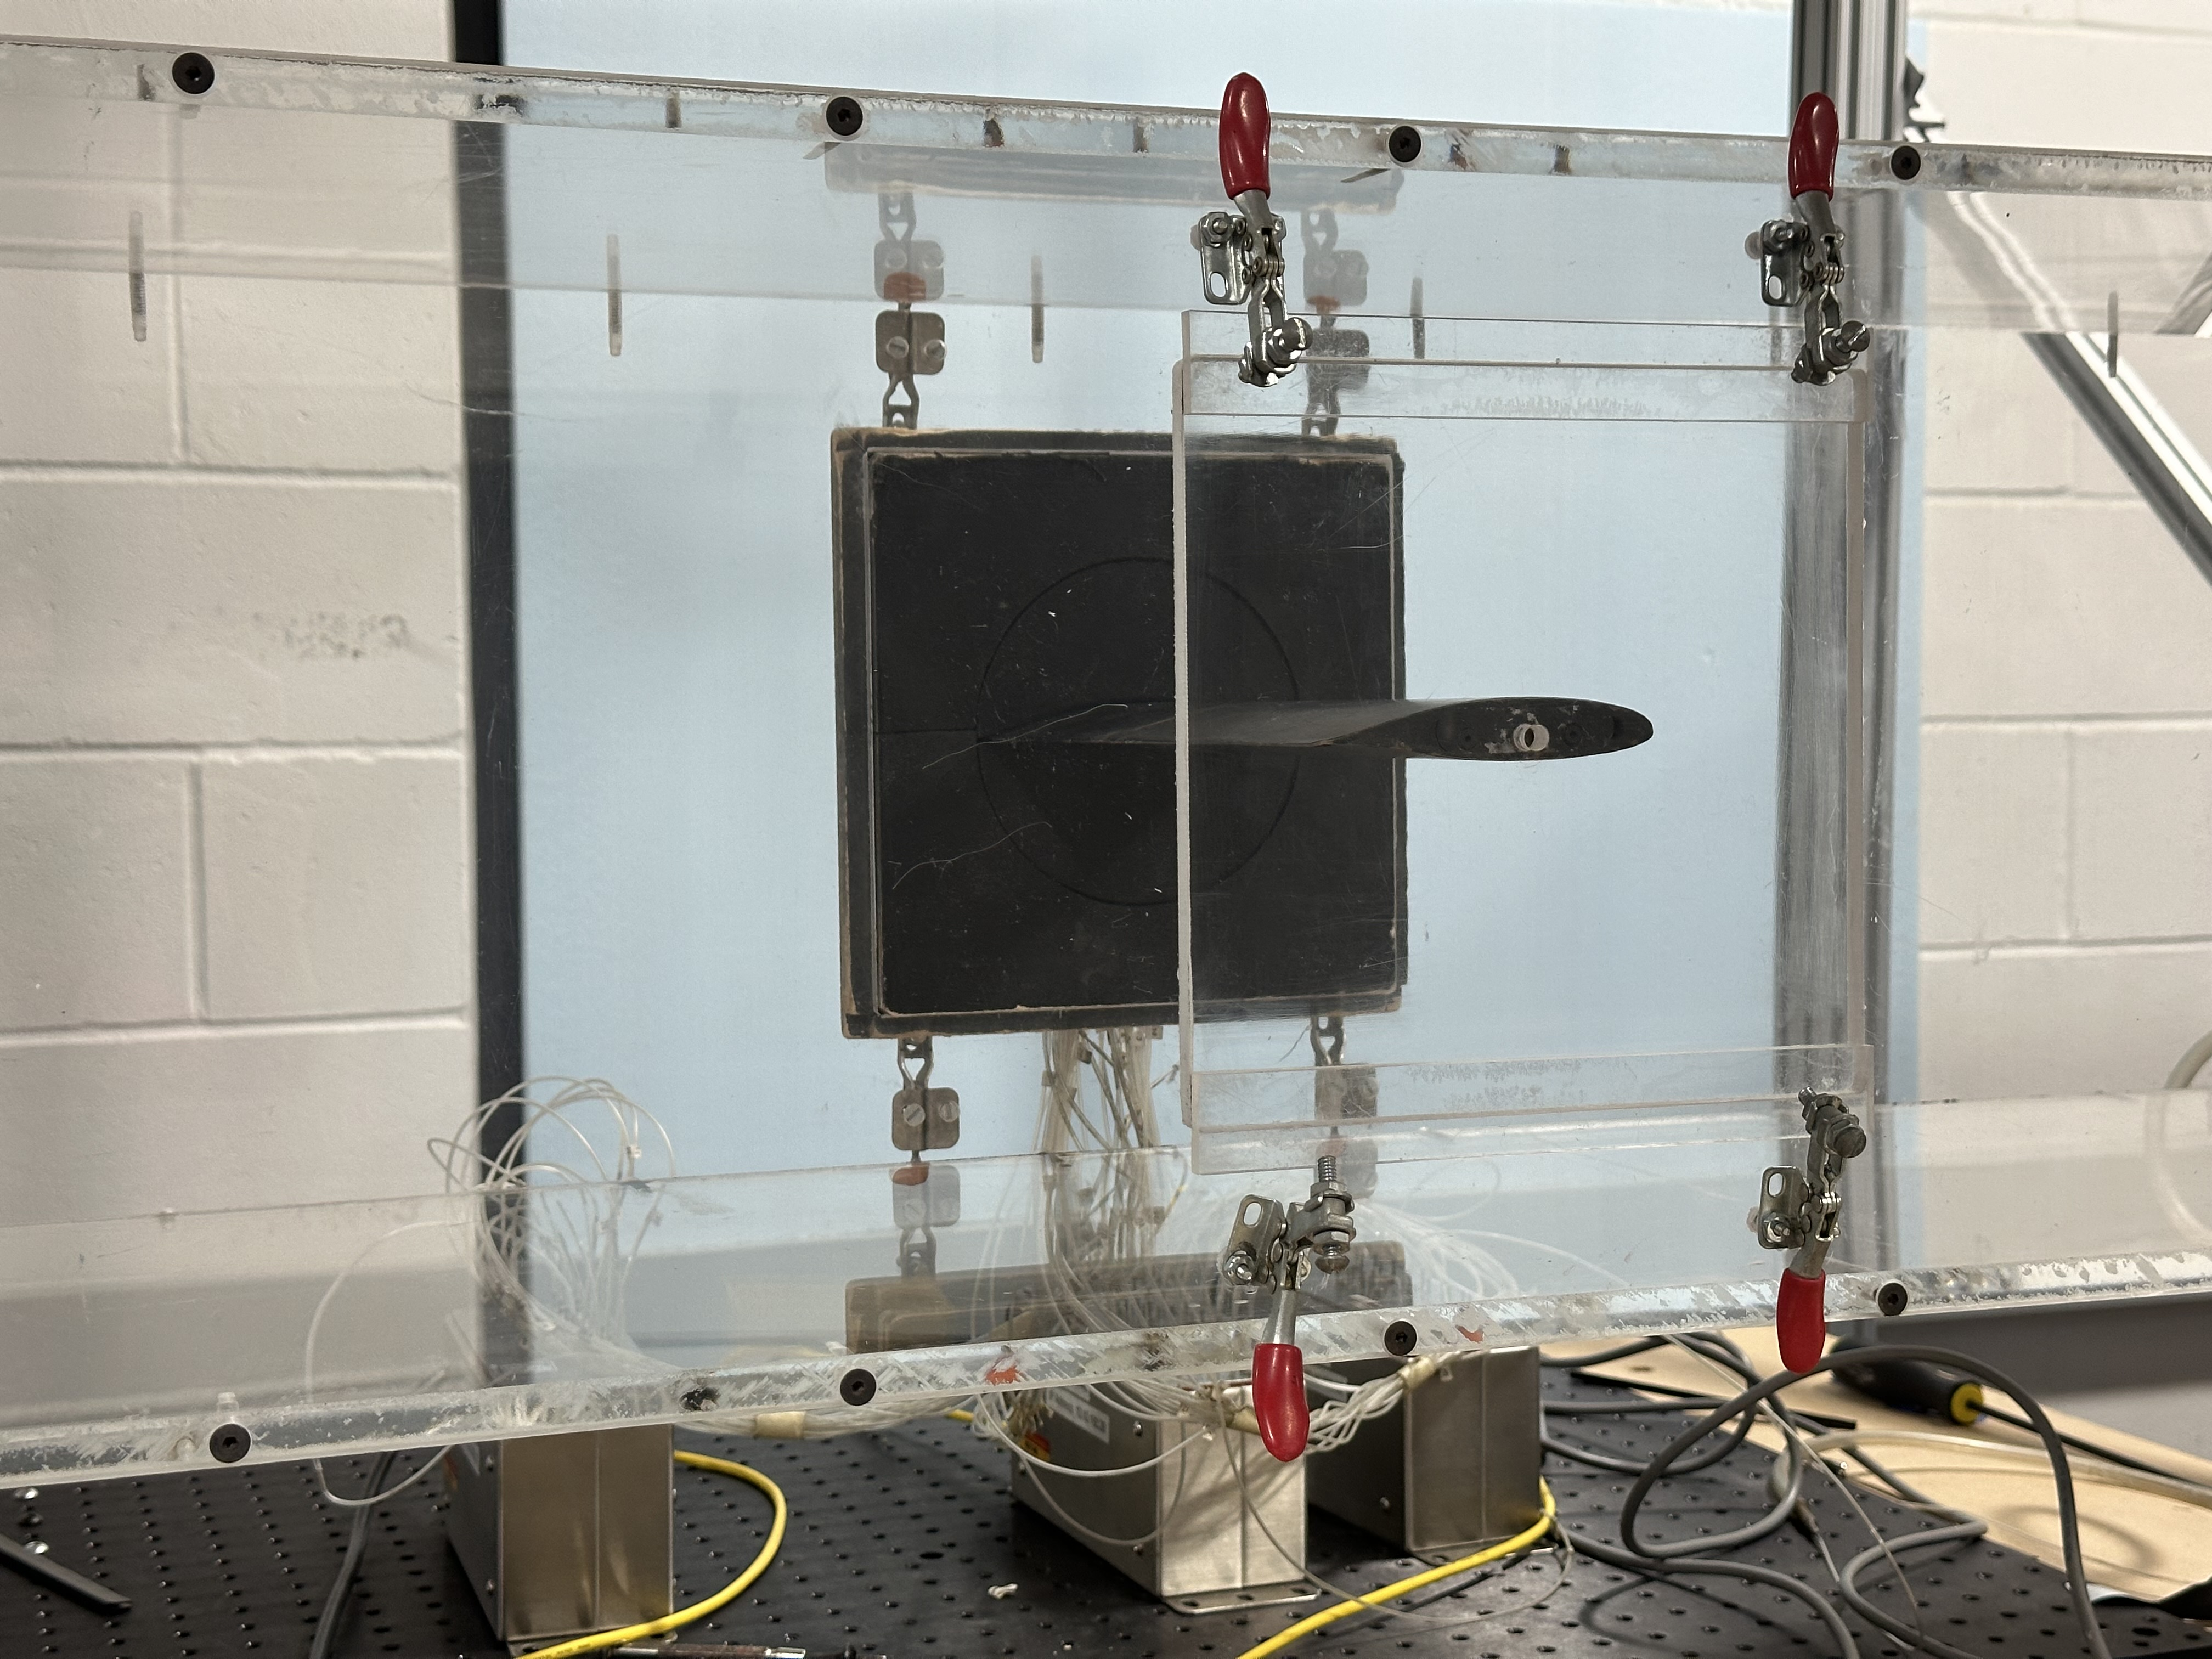
\includegraphics[width=0.75\linewidth]{Figures/IMG_3161.jpeg}
    \caption[Image of Airfoil in Test Section.]{Image of Airfoil in Test Section.}
    \label{fig: AirfoilTestSection_back}
\end{figure}

\begin{figure}[htpb]
    \centering
    \includegraphics[width=0.75\linewidth]{Figures/IMG_3163.jpeg}
    \caption[Image of the Scanivalve tester next to the test section.]{Image of the Scanivalve tester next to the test section.}
    \label{fig: scanivalve_top}
\end{figure}

\begin{figure}[htpb]
    \centering
    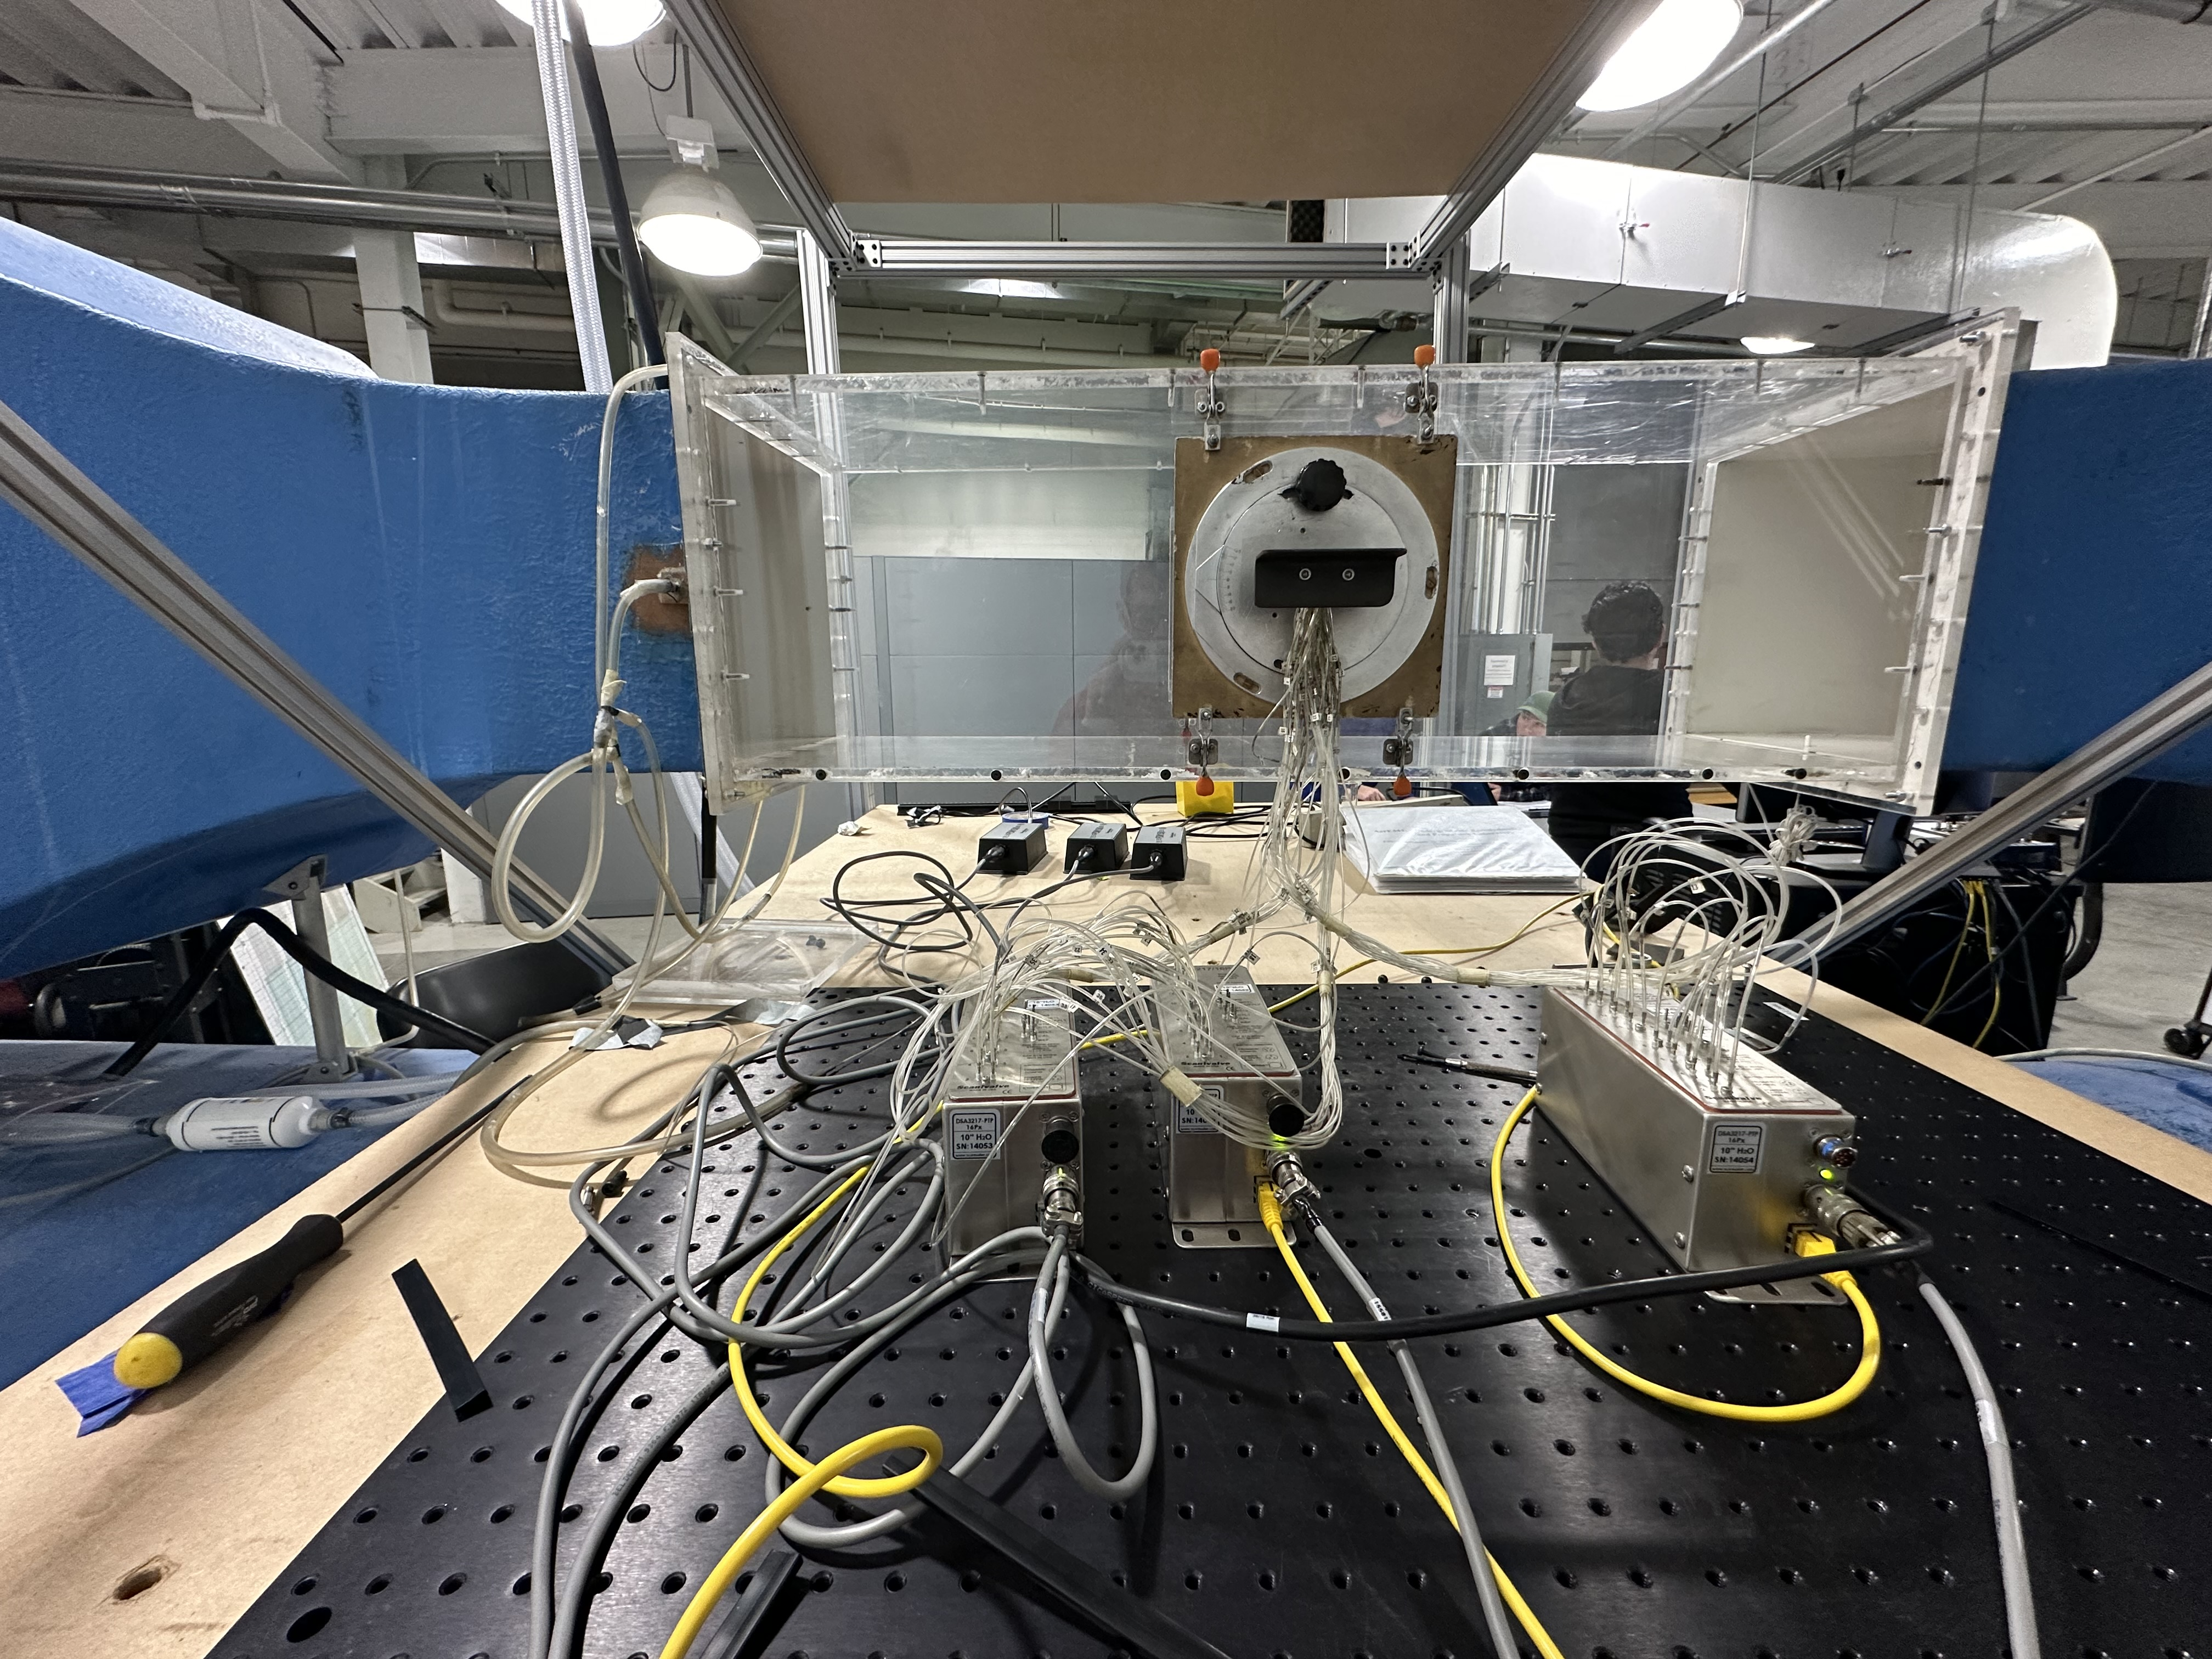
\includegraphics[width=0.75\linewidth]{Figures/IMG_3164.jpeg}
    \caption[Image of the Scanivalve tester next to the test section.]{Image of the Scanivalve tester next to the test section.}
    \label{fig: AirfoilTestSection_top}
\end{figure}